\documentclass[a4paper]{report}

%====================== PACKAGES ======================

\usepackage[french]{babel}
\usepackage[utf8]{inputenc}
%pour gérer les positionnement d'images
\usepackage{float}
\usepackage{amsmath}
\usepackage{graphicx}
\usepackage[colorinlistoftodos]{todonotes}
\usepackage{url}
%pour les informations sur un document compilé en PDF et les liens externes / internes
\usepackage{hyperref}
%pour la mise en page des tableaux
\usepackage{array}
\usepackage{tabularx}
%pour utiliser \floatbarrier
%\usepackage{placeins}
%\usepackage{floatrow}
%espacement entre les lignes
\usepackage{setspace}
%modifier la mise en page de l'abstract
\usepackage{abstract}
%police et mise en page (marges) du document
\usepackage[T1]{fontenc}
\usepackage[top=2cm, bottom=2cm, left=2cm, right=2cm]{geometry}
%Pour les galerie d'images
\usepackage{subfig}






% Default to the notebook output style




% Inherit from the specified cell style.





    \usepackage{adjustbox} % Used to constrain images to a maximum size
    \usepackage{color} % Allow colors to be defined
    \usepackage{enumerate} % Needed for markdown enumerations to work
    \usepackage{geometry} % Used to adjust the document margins
    \usepackage{amsmath} % Equations
    \usepackage{amssymb} % Equations
    \usepackage{eurosym} % defines \euro
    \usepackage[mathletters]{ucs} % Extended unicode (utf-8) support
    \usepackage{fancyvrb} % verbatim replacement that allows latex
    \usepackage{grffile} % extends the file name processing of package graphics
                         % to support a larger range
    % The hyperref package gives us a pdf with properly built
    % internal navigation ('pdf bookmarks' for the table of contents,
    % internal cross-reference links, web links for URLs, etc.)
    \usepackage{hyperref}
    \usepackage{longtable} % longtable support required by pandoc >1.10
    \usepackage{booktabs}  % table support for pandoc > 1.12.2
    \usepackage{ulem} % ulem is needed to support strikethroughs (\sout)




    \definecolor{orange}{cmyk}{0,0.4,0.8,0.2}
    \definecolor{darkorange}{rgb}{.71,0.21,0.01}
    \definecolor{darkgreen}{rgb}{.12,.54,.11}
    \definecolor{myteal}{rgb}{.26, .44, .56}
    \definecolor{gray}{gray}{0.45}
    \definecolor{lightgray}{gray}{.95}
    \definecolor{mediumgray}{gray}{.8}
    \definecolor{inputbackground}{rgb}{.95, .95, .85}
    \definecolor{outputbackground}{rgb}{.95, .95, .95}
    \definecolor{traceback}{rgb}{1, .95, .95}
    % ansi colors
    \definecolor{red}{rgb}{.6,0,0}
    \definecolor{green}{rgb}{0,.65,0}
    \definecolor{brown}{rgb}{0.6,0.6,0}
    \definecolor{blue}{rgb}{0,.145,.698}
    \definecolor{purple}{rgb}{.698,.145,.698}
    \definecolor{cyan}{rgb}{0,.698,.698}
    \definecolor{lightgray}{gray}{0.5}

    % bright ansi colors
    \definecolor{darkgray}{gray}{0.25}
    \definecolor{lightred}{rgb}{1.0,0.39,0.28}
    \definecolor{lightgreen}{rgb}{0.48,0.99,0.0}
    \definecolor{lightblue}{rgb}{0.53,0.81,0.92}
    \definecolor{lightpurple}{rgb}{0.87,0.63,0.87}
    \definecolor{lightcyan}{rgb}{0.5,1.0,0.83}

    % commands and environments needed by pandoc snippets
    % extracted from the output of `pandoc -s`
    \providecommand{\tightlist}{%
      \setlength{\itemsep}{0pt}\setlength{\parskip}{0pt}}
    \DefineVerbatimEnvironment{Highlighting}{Verbatim}{commandchars=\\\{\}}
    % Add ',fontsize=\small' for more characters per line
    \newenvironment{Shaded}{}{}
    \newcommand{\KeywordTok}[1]{\textcolor[rgb]{0.00,0.44,0.13}{\textbf{{#1}}}}
    \newcommand{\DataTypeTok}[1]{\textcolor[rgb]{0.56,0.13,0.00}{{#1}}}
    \newcommand{\DecValTok}[1]{\textcolor[rgb]{0.25,0.63,0.44}{{#1}}}
    \newcommand{\BaseNTok}[1]{\textcolor[rgb]{0.25,0.63,0.44}{{#1}}}
    \newcommand{\FloatTok}[1]{\textcolor[rgb]{0.25,0.63,0.44}{{#1}}}
    \newcommand{\CharTok}[1]{\textcolor[rgb]{0.25,0.44,0.63}{{#1}}}
    \newcommand{\StringTok}[1]{\textcolor[rgb]{0.25,0.44,0.63}{{#1}}}
    \newcommand{\CommentTok}[1]{\textcolor[rgb]{0.38,0.63,0.69}{\textit{{#1}}}}
    \newcommand{\OtherTok}[1]{\textcolor[rgb]{0.00,0.44,0.13}{{#1}}}
    \newcommand{\AlertTok}[1]{\textcolor[rgb]{1.00,0.00,0.00}{\textbf{{#1}}}}
    \newcommand{\FunctionTok}[1]{\textcolor[rgb]{0.02,0.16,0.49}{{#1}}}
    \newcommand{\RegionMarkerTok}[1]{{#1}}
    \newcommand{\ErrorTok}[1]{\textcolor[rgb]{1.00,0.00,0.00}{\textbf{{#1}}}}
    \newcommand{\NormalTok}[1]{{#1}}

    % Additional commands for more recent versions of Pandoc
    \newcommand{\ConstantTok}[1]{\textcolor[rgb]{0.53,0.00,0.00}{{#1}}}
    \newcommand{\SpecialCharTok}[1]{\textcolor[rgb]{0.25,0.44,0.63}{{#1}}}
    \newcommand{\VerbatimStringTok}[1]{\textcolor[rgb]{0.25,0.44,0.63}{{#1}}}
    \newcommand{\SpecialStringTok}[1]{\textcolor[rgb]{0.73,0.40,0.53}{{#1}}}
    \newcommand{\ImportTok}[1]{{#1}}
    \newcommand{\DocumentationTok}[1]{\textcolor[rgb]{0.73,0.13,0.13}{\textit{{#1}}}}
    \newcommand{\AnnotationTok}[1]{\textcolor[rgb]{0.38,0.63,0.69}{\textbf{\textit{{#1}}}}}
    \newcommand{\CommentVarTok}[1]{\textcolor[rgb]{0.38,0.63,0.69}{\textbf{\textit{{#1}}}}}
    \newcommand{\VariableTok}[1]{\textcolor[rgb]{0.10,0.09,0.49}{{#1}}}
    \newcommand{\ControlFlowTok}[1]{\textcolor[rgb]{0.00,0.44,0.13}{\textbf{{#1}}}}
    \newcommand{\OperatorTok}[1]{\textcolor[rgb]{0.40,0.40,0.40}{{#1}}}
    \newcommand{\BuiltInTok}[1]{{#1}}
    \newcommand{\ExtensionTok}[1]{{#1}}
    \newcommand{\PreprocessorTok}[1]{\textcolor[rgb]{0.74,0.48,0.00}{{#1}}}
    \newcommand{\AttributeTok}[1]{\textcolor[rgb]{0.49,0.56,0.16}{{#1}}}
    \newcommand{\InformationTok}[1]{\textcolor[rgb]{0.38,0.63,0.69}{\textbf{\textit{{#1}}}}}
    \newcommand{\WarningTok}[1]{\textcolor[rgb]{0.38,0.63,0.69}{\textbf{\textit{{#1}}}}}


    % Define a nice break command that doesn't care if a line doesn't already
    % exist.
    \def\br{\hspace*{\fill} \\* }
    % Math Jax compatability definitions
    \def\gt{>}
    \def\lt{<}
    % Document parameters
    \title{Untitled}




    % Pygments definitions

\makeatletter
\def\PY@reset{\let\PY@it=\relax \let\PY@bf=\relax%
    \let\PY@ul=\relax \let\PY@tc=\relax%
    \let\PY@bc=\relax \let\PY@ff=\relax}
\def\PY@tok#1{\csname PY@tok@#1\endcsname}
\def\PY@toks#1+{\ifx\relax#1\empty\else%
    \PY@tok{#1}\expandafter\PY@toks\fi}
\def\PY@do#1{\PY@bc{\PY@tc{\PY@ul{%
    \PY@it{\PY@bf{\PY@ff{#1}}}}}}}
\def\PY#1#2{\PY@reset\PY@toks#1+\relax+\PY@do{#2}}

\expandafter\def\csname PY@tok@o\endcsname{\def\PY@tc##1{\textcolor[rgb]{0.40,0.40,0.40}{##1}}}
\expandafter\def\csname PY@tok@cp\endcsname{\def\PY@tc##1{\textcolor[rgb]{0.74,0.48,0.00}{##1}}}
\expandafter\def\csname PY@tok@vg\endcsname{\def\PY@tc##1{\textcolor[rgb]{0.10,0.09,0.49}{##1}}}
\expandafter\def\csname PY@tok@no\endcsname{\def\PY@tc##1{\textcolor[rgb]{0.53,0.00,0.00}{##1}}}
\expandafter\def\csname PY@tok@mi\endcsname{\def\PY@tc##1{\textcolor[rgb]{0.40,0.40,0.40}{##1}}}
\expandafter\def\csname PY@tok@ss\endcsname{\def\PY@tc##1{\textcolor[rgb]{0.10,0.09,0.49}{##1}}}
\expandafter\def\csname PY@tok@s\endcsname{\def\PY@tc##1{\textcolor[rgb]{0.73,0.13,0.13}{##1}}}
\expandafter\def\csname PY@tok@mf\endcsname{\def\PY@tc##1{\textcolor[rgb]{0.40,0.40,0.40}{##1}}}
\expandafter\def\csname PY@tok@gu\endcsname{\let\PY@bf=\textbf\def\PY@tc##1{\textcolor[rgb]{0.50,0.00,0.50}{##1}}}
\expandafter\def\csname PY@tok@vc\endcsname{\def\PY@tc##1{\textcolor[rgb]{0.10,0.09,0.49}{##1}}}
\expandafter\def\csname PY@tok@sb\endcsname{\def\PY@tc##1{\textcolor[rgb]{0.73,0.13,0.13}{##1}}}
\expandafter\def\csname PY@tok@cs\endcsname{\let\PY@it=\textit\def\PY@tc##1{\textcolor[rgb]{0.25,0.50,0.50}{##1}}}
\expandafter\def\csname PY@tok@kt\endcsname{\def\PY@tc##1{\textcolor[rgb]{0.69,0.00,0.25}{##1}}}
\expandafter\def\csname PY@tok@gd\endcsname{\def\PY@tc##1{\textcolor[rgb]{0.63,0.00,0.00}{##1}}}
\expandafter\def\csname PY@tok@kp\endcsname{\def\PY@tc##1{\textcolor[rgb]{0.00,0.50,0.00}{##1}}}
\expandafter\def\csname PY@tok@sx\endcsname{\def\PY@tc##1{\textcolor[rgb]{0.00,0.50,0.00}{##1}}}
\expandafter\def\csname PY@tok@gr\endcsname{\def\PY@tc##1{\textcolor[rgb]{1.00,0.00,0.00}{##1}}}
\expandafter\def\csname PY@tok@gp\endcsname{\let\PY@bf=\textbf\def\PY@tc##1{\textcolor[rgb]{0.00,0.00,0.50}{##1}}}
\expandafter\def\csname PY@tok@il\endcsname{\def\PY@tc##1{\textcolor[rgb]{0.40,0.40,0.40}{##1}}}
\expandafter\def\csname PY@tok@nd\endcsname{\def\PY@tc##1{\textcolor[rgb]{0.67,0.13,1.00}{##1}}}
\expandafter\def\csname PY@tok@m\endcsname{\def\PY@tc##1{\textcolor[rgb]{0.40,0.40,0.40}{##1}}}
\expandafter\def\csname PY@tok@nt\endcsname{\let\PY@bf=\textbf\def\PY@tc##1{\textcolor[rgb]{0.00,0.50,0.00}{##1}}}
\expandafter\def\csname PY@tok@cm\endcsname{\let\PY@it=\textit\def\PY@tc##1{\textcolor[rgb]{0.25,0.50,0.50}{##1}}}
\expandafter\def\csname PY@tok@nl\endcsname{\def\PY@tc##1{\textcolor[rgb]{0.63,0.63,0.00}{##1}}}
\expandafter\def\csname PY@tok@kn\endcsname{\let\PY@bf=\textbf\def\PY@tc##1{\textcolor[rgb]{0.00,0.50,0.00}{##1}}}
\expandafter\def\csname PY@tok@gs\endcsname{\let\PY@bf=\textbf}
\expandafter\def\csname PY@tok@kc\endcsname{\let\PY@bf=\textbf\def\PY@tc##1{\textcolor[rgb]{0.00,0.50,0.00}{##1}}}
\expandafter\def\csname PY@tok@nf\endcsname{\def\PY@tc##1{\textcolor[rgb]{0.00,0.00,1.00}{##1}}}
\expandafter\def\csname PY@tok@gi\endcsname{\def\PY@tc##1{\textcolor[rgb]{0.00,0.63,0.00}{##1}}}
\expandafter\def\csname PY@tok@ow\endcsname{\let\PY@bf=\textbf\def\PY@tc##1{\textcolor[rgb]{0.67,0.13,1.00}{##1}}}
\expandafter\def\csname PY@tok@ne\endcsname{\let\PY@bf=\textbf\def\PY@tc##1{\textcolor[rgb]{0.82,0.25,0.23}{##1}}}
\expandafter\def\csname PY@tok@s2\endcsname{\def\PY@tc##1{\textcolor[rgb]{0.73,0.13,0.13}{##1}}}
\expandafter\def\csname PY@tok@nb\endcsname{\def\PY@tc##1{\textcolor[rgb]{0.00,0.50,0.00}{##1}}}
\expandafter\def\csname PY@tok@s1\endcsname{\def\PY@tc##1{\textcolor[rgb]{0.73,0.13,0.13}{##1}}}
\expandafter\def\csname PY@tok@cpf\endcsname{\let\PY@it=\textit\def\PY@tc##1{\textcolor[rgb]{0.25,0.50,0.50}{##1}}}
\expandafter\def\csname PY@tok@nn\endcsname{\let\PY@bf=\textbf\def\PY@tc##1{\textcolor[rgb]{0.00,0.00,1.00}{##1}}}
\expandafter\def\csname PY@tok@gt\endcsname{\def\PY@tc##1{\textcolor[rgb]{0.00,0.27,0.87}{##1}}}
\expandafter\def\csname PY@tok@c1\endcsname{\let\PY@it=\textit\def\PY@tc##1{\textcolor[rgb]{0.25,0.50,0.50}{##1}}}
\expandafter\def\csname PY@tok@sr\endcsname{\def\PY@tc##1{\textcolor[rgb]{0.73,0.40,0.53}{##1}}}
\expandafter\def\csname PY@tok@na\endcsname{\def\PY@tc##1{\textcolor[rgb]{0.49,0.56,0.16}{##1}}}
\expandafter\def\csname PY@tok@w\endcsname{\def\PY@tc##1{\textcolor[rgb]{0.73,0.73,0.73}{##1}}}
\expandafter\def\csname PY@tok@nc\endcsname{\let\PY@bf=\textbf\def\PY@tc##1{\textcolor[rgb]{0.00,0.00,1.00}{##1}}}
\expandafter\def\csname PY@tok@nv\endcsname{\def\PY@tc##1{\textcolor[rgb]{0.10,0.09,0.49}{##1}}}
\expandafter\def\csname PY@tok@gh\endcsname{\let\PY@bf=\textbf\def\PY@tc##1{\textcolor[rgb]{0.00,0.00,0.50}{##1}}}
\expandafter\def\csname PY@tok@bp\endcsname{\def\PY@tc##1{\textcolor[rgb]{0.00,0.50,0.00}{##1}}}
\expandafter\def\csname PY@tok@ch\endcsname{\let\PY@it=\textit\def\PY@tc##1{\textcolor[rgb]{0.25,0.50,0.50}{##1}}}
\expandafter\def\csname PY@tok@k\endcsname{\let\PY@bf=\textbf\def\PY@tc##1{\textcolor[rgb]{0.00,0.50,0.00}{##1}}}
\expandafter\def\csname PY@tok@sc\endcsname{\def\PY@tc##1{\textcolor[rgb]{0.73,0.13,0.13}{##1}}}
\expandafter\def\csname PY@tok@kr\endcsname{\let\PY@bf=\textbf\def\PY@tc##1{\textcolor[rgb]{0.00,0.50,0.00}{##1}}}
\expandafter\def\csname PY@tok@ge\endcsname{\let\PY@it=\textit}
\expandafter\def\csname PY@tok@se\endcsname{\let\PY@bf=\textbf\def\PY@tc##1{\textcolor[rgb]{0.73,0.40,0.13}{##1}}}
\expandafter\def\csname PY@tok@mo\endcsname{\def\PY@tc##1{\textcolor[rgb]{0.40,0.40,0.40}{##1}}}
\expandafter\def\csname PY@tok@err\endcsname{\def\PY@bc##1{\setlength{\fboxsep}{0pt}\fcolorbox[rgb]{1.00,0.00,0.00}{1,1,1}{\strut ##1}}}
\expandafter\def\csname PY@tok@c\endcsname{\let\PY@it=\textit\def\PY@tc##1{\textcolor[rgb]{0.25,0.50,0.50}{##1}}}
\expandafter\def\csname PY@tok@mb\endcsname{\def\PY@tc##1{\textcolor[rgb]{0.40,0.40,0.40}{##1}}}
\expandafter\def\csname PY@tok@vi\endcsname{\def\PY@tc##1{\textcolor[rgb]{0.10,0.09,0.49}{##1}}}
\expandafter\def\csname PY@tok@sd\endcsname{\let\PY@it=\textit\def\PY@tc##1{\textcolor[rgb]{0.73,0.13,0.13}{##1}}}
\expandafter\def\csname PY@tok@go\endcsname{\def\PY@tc##1{\textcolor[rgb]{0.53,0.53,0.53}{##1}}}
\expandafter\def\csname PY@tok@kd\endcsname{\let\PY@bf=\textbf\def\PY@tc##1{\textcolor[rgb]{0.00,0.50,0.00}{##1}}}
\expandafter\def\csname PY@tok@ni\endcsname{\let\PY@bf=\textbf\def\PY@tc##1{\textcolor[rgb]{0.60,0.60,0.60}{##1}}}
\expandafter\def\csname PY@tok@mh\endcsname{\def\PY@tc##1{\textcolor[rgb]{0.40,0.40,0.40}{##1}}}
\expandafter\def\csname PY@tok@sh\endcsname{\def\PY@tc##1{\textcolor[rgb]{0.73,0.13,0.13}{##1}}}
\expandafter\def\csname PY@tok@si\endcsname{\let\PY@bf=\textbf\def\PY@tc##1{\textcolor[rgb]{0.73,0.40,0.53}{##1}}}

\def\PYZbs{\char`\\}
\def\PYZus{\char`\_}
\def\PYZob{\char`\{}
\def\PYZcb{\char`\}}
\def\PYZca{\char`\^}
\def\PYZam{\char`\&}
\def\PYZlt{\char`\<}
\def\PYZgt{\char`\>}
\def\PYZsh{\char`\#}
\def\PYZpc{\char`\%}
\def\PYZdl{\char`\$}
\def\PYZhy{\char`\-}
\def\PYZsq{\char`\'}
\def\PYZdq{\char`\"}
\def\PYZti{\char`\~}
% for compatibility with earlier versions
\def\PYZat{@}
\def\PYZlb{[}
\def\PYZrb{]}
\makeatother


    % Exact colors from NB
    \definecolor{incolor}{rgb}{0.0, 0.0, 0.5}
    \definecolor{outcolor}{rgb}{0.545, 0.0, 0.0}




    % Prevent overflowing lines due to hard-to-break entities
    \sloppy
    % Setup hyperref package
    \hypersetup{
      breaklinks=true,  % so long urls are correctly broken across lines
      colorlinks=true,
      urlcolor=blue,
      linkcolor=darkorange,
      citecolor=darkgreen,
      }
    % Slightly bigger margins than the latex defaults

    \geometry{verbose,tmargin=1in,bmargin=1in,lmargin=1in,rmargin=1in}








%====================== INFORMATION ET REGLES ======================
%rajouter les numérotation pour les \paragraphe et \subparagraphe
\setcounter{secnumdepth}{4}
\setcounter{tocdepth}{4}

\hypersetup{							% Information sur le document
pdfauthor = {Premier Auteur,
			Deuxième Auteur,
			Troisième Auteur,
    		Quatrième Auteur},			% Auteurs
pdftitle = {Dominion datamining -
			Mémoire du projet},			% Titre du document
pdfsubject = {Mémoire de Projet},		% Sujet
pdfkeywords = {Tag1, Tag2, Tag3, ...},	% Mots-clefs
pdfstartview={FitH}}					% ajuste la page à la largueur de l'écran
%pdfcreator = {MikTeX},% Logiciel qui a crée le document
%pdfproducer = {}} % Société avec produit le logiciel

%======================== DEBUT DU DOCUMENT ========================

\begin{document}

%régler l'espacement entre les lignes
\newcommand{\HRule}{\rule{\linewidth}{0.5mm}}

%page de garde
\begin{titlepage}
\begin{center}

% Upper part of the page. The '~' is needed because only works if a paragraph has started.

\includegraphics[width=0.35\textwidth]{./logo}~\\[1cm]

\textsc{\LARGE Université ou Entreprise}\\[1.5cm]

\textsc{\Large }\\[0.5cm]

% Title
\HRule \\[0.4cm]

{\huge \bfseries Nom du Projet\\
Sujet du Projet \\[0.4cm] }

\HRule \\[1.5cm]

% Author and supervisor
\begin{minipage}{0.4\textwidth}
\begin{flushleft} \large
\emph{Auteur:}\\
Premier \textsc{Auteur}\\
Deuxième \textsc{Auteur}\\
Troisième \textsc{Auteur}\\
Quatrième \textsc{Auteur}
\end{flushleft}
\end{minipage}
\begin{minipage}{0.4\textwidth}
\begin{flushright} \large
\emph{Client:} \\
Prénom \textsc{Nom}\\
\emph{Référent:} \\
Prénom \textsc{Nom}
\end{flushright}
\end{minipage}

\vfill

% Bottom of the page
{\large \today}

\end{center}
\end{titlepage}

%page blanche
\newpage
~
%ne pas numéroter cette page
\thispagestyle{empty}
\newpage

\renewcommand{\abstractnamefont}{\normalfont\Large\bfseries}
%\renewcommand{\abstracttextfont}{\normalfont\Huge}

\begin{abstract}
\hskip7mm

\begin{spacing}{1.3}

Lorem ipsum dolor sit amet, consectetur adipiscing elit. Sed non risus. Suspendisse lectus tortor, dignissim sit amet, adipiscing nec, ultricies sed, dolor. Cras elementum ultrices diam. Maecenas ligula massa, varius a, semper congue, euismod non, mi. Proin porttitor, orci nec nonummy molestie, enim est eleifend mi, non fermentum diam nisl sit amet erat. Duis semper. Duis arcu massa, scelerisque vitae, consequat in, pretium a, enim. Pellentesque congue. Ut in risus volutpat libero pharetra tempor. Cras vestibulum bibendum augue. Praesent egestas leo in pede. Praesent blandit odio eu enim. Pellentesque sed dui ut augue blandit sodales. Vestibulum ante ipsum primis in faucibus orci luctus et ultrices posuere cubilia Curae; Aliquam nibh. Mauris ac mauris sed pede pellentesque fermentum. Maecenas adipiscing ante non diam sodales hendrerit. Ut velit mauris, egestas sed, gravida nec, ornare ut, mi. Aenean ut orci vel massa suscipit pulvinar. Nulla sollicitudin. Fusce varius, ligula non tempus aliquam, nunc turpis ullamcorper nibh, in tempus sapien eros vitae ligula. Pellentesque rhoncus nunc et augue. Integer id felis. Curabitur aliquet pellentesque diam. Integer quis metus vitae elit lobortis egestas. Lorem ipsum dolor sit amet, consectetuer adipiscing elit. Morbi vel erat non mauris convallis vehicula. Nulla et sapien. Integer tortor tellus, aliquam faucibus, convallis id, congue eu, quam. Mauris ullamcorper felis vitae erat. Proin feugiat, augue non elementum posuere, metus purus iaculis lectus, et tristique ligula justo vitae magna. Aliquam convallis sollicitudin purus. Praesent aliquam, enim at fermentum mollis, ligula massa adipiscing nisl, ac euismod nibh nisl eu lectus. Fusce vulputate sem at sapien. Vivamus leo. Aliquam euismod libero eu enim. Nulla nec felis sed leo placerat imperdiet. Aenean suscipit nulla in justo. Suspendisse cursus rutrum augue. Nulla tincidunt tincidunt mi. Curabitur iaculis, lorem vel rhoncus faucibus, felis magna fermentum augue, et ultricies lacus lorem varius purus. Curabitur eu amet.

\end{spacing}
\end{abstract}


\tableofcontents
\thispagestyle{empty}
\setcounter{page}{0}
%ne pas numéroter le sommaire

\newpage

%espacement entre les lignes d'un tableau
\renewcommand{\arraystretch}{1.5}

%====================== INCLUSION DES PARTIES ======================

~
\thispagestyle{empty}
%recommencer la numérotation des pages à "1"
\setcounter{page}{0}
\newpage

\chapter{Présentation du projet}

Le jeu de cartes \textit{Dominion} a été mis à disposition sur un serveur de jeu d'octobre 2010 à mars 2013. Les parties effectuées via ce serveur ont été enregistrées dans des \textit{logs} qui mémorisaient toutes les actions des joueurs ; ces \textit{logs} ont été mis à disposition du public. Mais ces enregistrements n'ont pas conservé un certain nombre d'informations ayant un rapport avec les décisions prises par les joueurs.
\newline Un wiki relatif au jeu a été élaboré, et propose des avis d'experts comme aide à la décision pour les joueurs : il propose des conseils, notamment au niveau stratégique. Le but de ce projet, proposé par Yvan Le Borgne, chercheur au Labri, est de traiter ces \textit{logs} (soit plus de 12 millions de parties) afin de répondre à plusieurs interrogations. Il s'agira principalement de comparer Les données recueillies aux préconisations de ce wiki,afin de valider, à travers les contenus des parties, l'éventuelle efficacité des avis et suggestions fournies par les experts. A tout le moins, on cherchera à élaborer des outils de validation présentant une efficacité suffisante.
\newline A cet effet, le projet a pour but de créer une base de données recensant les parties puis un travail d'analyse sera effectuée à partir de celle-ci.
Pour cela notre programme devra tout d'abord extraire les données présentes dans les logs, car ceux-ci sont trop volumineux et trop compliqués à utiliser directement (structure non standardisée). Il s'agira de mettre au point des structures de données permettant de stocker les données de manière plus efficace. Une manière simple de représenter les données extraites et analysées sera proposée à l'utilisateur.
Par ailleurs, il manque des informations dans les enregistrements (\textit{logs}). On cherchera à trouver par quelle méthode on peut les reconstituer et de les mettre dans un format contenant toutes les informations.
En outre, on cherchera à optimiser les opérations menées dans l'analyse des donnnées, en recherchant le meilleur équilibre possible entre la mémorisation des recherches et le re-calcul.
Enfin, on esssaiera de déterminer quelle stratégie a été utilisée dans chaque partie. Voire de faire émerger les changements de stratégie en cours de partie. Si on prend par exemple une des stratégies (la \textit{Penultimate Province Rule}) peut on détecter à quel moment cette règle a été appliquée ou contournée ? ou qui a mis au point cette stratégie ? (découverte qui pourrait permettre d'organiser un classement des joueurs les plus performants) (une sorte de ELO demandé par le client). Dans la mesure où on parviendrait à mettre au point un nombre suffisant de ces démarches stratégiques, il s'agirait de déterminer le processus habituel d'apprentissage des joueurs.

\section{Règles du jeu}
Chaque joueur possède un deck de cartes et a accès à un <<marché>> ou différentes cartes d'action sont disponible. Il y a également une pile de cartes de victoires.
\newline Les joueurs commencent avec un deck contenant uniquement des cartes de monnaie permettant d'acheter les autres cartes mises à la disposition des joueurs. Les joueurs commencent leur tour avec 5 cartes en main et le tour d'un joueur se déroule en deux phases, premièrement la phase d'action, le joueur peut jouer une carte d'action, puis une phase d'achat ou le joueur peut acheter des cartes du marché, des cartes de monnaie ou des cartes de victoires.
\newline La partie se termine dans deux cas, si la réserve de cartes <<Province>> (carte de victoire au score le plus élevé) est vide ou bien si 3 piles du marché sont vides. Quand la partie est terminée, les points de victoires (découlant des cartes de victoire) de chaque deck sont comptés et le vainqueur est celui qui à la meilleur score.


\section{Sujet}

Bla(cf. fig. 1.1)\\

%inclusion d'une mage dans le document
\begin{figure}[!h]
\begin{center}
%taille de l'image en largeur
%remplacer "width" par "height" pour régler la hauteur
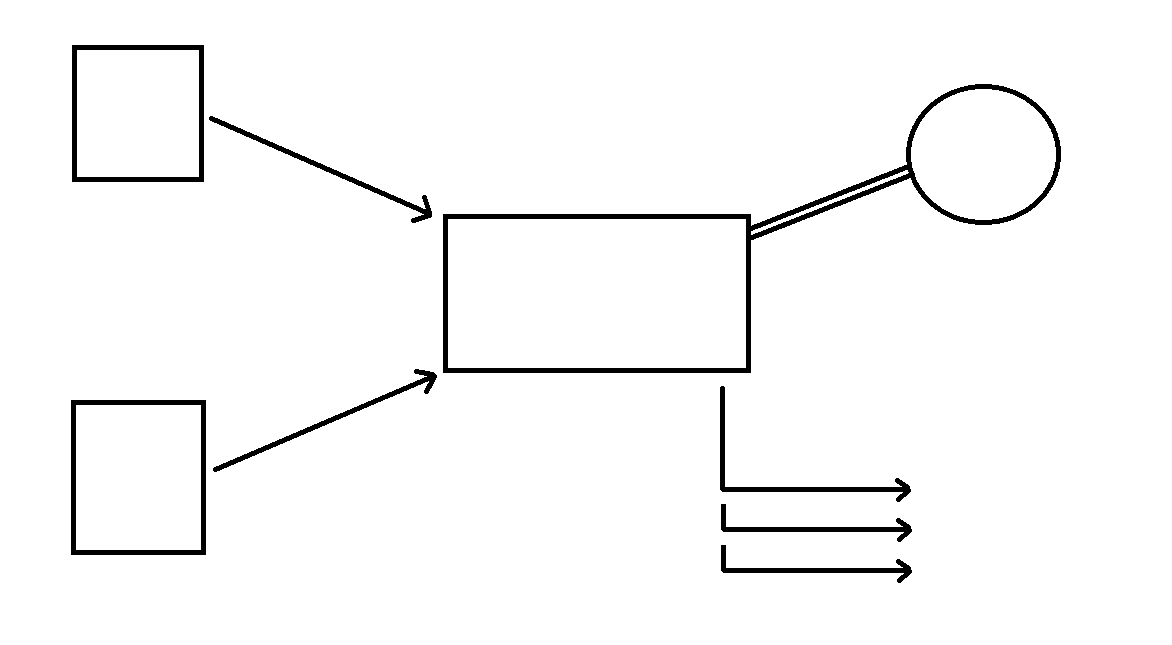
\includegraphics[width=15cm]{presentation/schema}
\end{center}
%légende de l'image
\caption{Schéma descriptif}
\end{figure}

%Contenu de la note précédemment marquée avec \footnotemark
\footnotetext{Note bas de page "intro"}

Bla
%retour à la ligne (alinea)

Bla\\
%saut de paragraphe

Bla

\newpage

\section{Problématique soulevée}

Bla

\begin{center}
Problématique du sujet
\end{center}

\section{Hypothèse de solution}

%Quoi :
Bla\\

Voici une liste :
\begin{itemize}
\item item 1;
\item item 2;
\item item 3;
\item item 4.
\end{itemize}

Bla\\

%Comment :
Bla

Bla\footnotemark\\

%Detail :
Bla(cf. ref. \cite{cite6}).
%citation référencé dans le document "bibliographie.bib" inclus à la fin du document

\footnotetext{Note bas de page "bla"}


\chapter{Analyse de l'existant}

\section{Description des données}
Les données qui ont été fournies par le client avaient été compressées au format \textit{tar.bz2}. Un fichier contenait chaque journée de Logs, et le total des données compressées se montait à 13 Go. Une fois décompressées, les données faisaient un total de 400 Go. 
Chaque Log est au format html. 
Chaque \textit{Log} doit contenir : 
\begin{itemize}
\item une en-tête contenant le numéro du jeu, et le gagnant.
\item un résumé du match contenant les cartes utilisées pendant le match, et comment le match a fini.
\item un résumé du joueur, contenant toutes les "cartes de victoire" du joueur, le \textit{deck}, les points et le nombre de tours joués.
\item l'enregistrement des différentes étapes du jeu, qui contient tous les détails des mouvements effectués par les joueurs au cours de la partie.  
\end{itemize}

\section{Incohérences dans les données}
Les \textit{logs} présentent des incohérences qui peuvent créer des problèmes pour le développement du parser ; quelques-un des problèmes rencontrés ont été les suivants : 
\begin{itemize}
\item \textbf{Numéro de \textit{log}} : la numérotation des logs n'était pas unique, ce qui voulait dire qu'on ne pouvait pas l'utiliser pour identifier un log.
\item \textbf{Nom d'utilisateur} : les logs font apparaître qu'il n'y avait pas de restriction quant aux noms des joueurs, et un certain nombre de noms de joueurs contiennent des mots-clés et utilisent des caractères spéciaux qui entrent en conflit avec le parser. 
\item \textbf{Données manquantes} : dans quelques logs, il manque une partie des données(comme par exemple l'en-tête, le résumé du joueur, etc...)
\item \textbf{Format du \textit{log}} : la syntaxe utilisée pour saisir les \textit{logs} n'est pas cohérente, et offre des différences entre différents \textit{logs}
\item \textbf{Compression des données} : comme les données sont compressées, et que le matériel fourni pour travailler sur le projet ne peut gérer les données une fois décompressées, il faudra travailler sur le projet avec des données compressées. Un premier essai de décompression a montré qu'il fallait un minimum de 4 heures pour tout décompresser. Il allait falloir en outre décompresser par tranches et effacer les contenus au fur et à mesure pour pouvoir fonctionner avec le matériel disponible. 
\end{itemize}

\section{Goko Dominion-tools}

Goko-dominion-tools est le principal outil disponible pour exploiter les logs, cet outil permet essentiellement de parser des logs bruts. Les fonctionnalités offertes par cet outil sont très proches de ce que nous voulons proposer, notamment un parsing de logs, une recherche dans ces logs et un classement. Le programme est écrit en python et est disponible sur github.

%\section{Bilan récapitulatif}

%Voici un tableau (cf. fig. 2.1) récapitulatif de notre analyse de l'existant...\\

%tableau centré à taille variable qui s'ajuste automatiquement suivant la longueur du contenu
%\begin{figure}[!h]
%\begin{center}
%\begin{tabular}{|l|l|l|l|l|}
%  \hline
%  Solution & Critère 1 & Critère 2 & Critère 3 & Critère 4\\
%  \hline
%  Solution 1(cf. ref. \cite{cite0}) & Oui & Oui & Oui & Oui \\
%  Solution 2(cf. ref. \cite{cite1}) & Oui & Oui & Oui & Non \\
%  Solution 3(cf. ref. \cite{cite2}) & Oui (sauf telle chose) & Non & Non & Oui\\
%  Solution 4(cf. ref. \cite{cite3}) & Oui& Non & Oui & Non\\
%  Solution 5(cf. ref. \cite{cite4}) & Oui (uniquement ceux-ci) & Non & Oui & Non\\
%  \hline
%\end{tabular}
%\end{center}
%\caption{Tableau récapitulatif des solutions}
%\end{figure}

 
\chapter{Analyse des besoins}


Comme on l'a vu dans l'approche théorique du \textit{Data Mining}, comme dans le cas de tout projet d'ailleurs, la définition des besoins est une étape cruciale du démarrage de l'activité. On va donc évoquer tout d'abord les besoins fonctionnels, puis les besoins non-fonctionnels.


\section{Besoins fonctionnels} 
Les besoins fonctionnels sont ceux qui permettent de remplir les conditions du cahier des charges ; ils sont incontournables. Il s'agit donc ici de voir comment on va répondre à la demande formulée à l'origine du projet.

\section{Interface utilisateur}
L'interface utilisateur se compose d'une bilibliothèque qui permettra à l'utilisateur d'exploiter les données récupérées par le parser. L'utilisateur pourra appeler les fonctions proposées par le programme ou bien écrire ses propres fonctions et les appliquer aux données.

\subsection{Se connecter à la base de données orientée documents}

\paragraph*{Description et piorité}

\textbf{Niveau de priorité = haute}

Cette librairie offrera des fonctions simples d'accès en lecture/écriture sur la base de données, de ce fait cette librairie pourra:
\begin{itemize}
\item récupérer un log ou les informations générales d'un joueur
\item mettre à jour les données relatives à un log ou aux informations générales d'un joueur
\item créer de nouvelles données issues des analyses effectuées
\end{itemize}

\subsection{Outils d'analyse}

\paragraph*{Description et piorité}

\textbf{Niveau de priorité = haute}

Une seconde librairie proposera une solution à l'utilisateur pour effectuer des analyses prédéfinies sur les données récupérées ainsi qu'un moyen d'appliquer de manière générale une analyse créée par l'utilisateur. Cette librairie pourra donc:
\begin{itemize}
\item appliquer une fonction spécifiée par l'utilisateur aux logs récupérés par une requète de l'utilisateur. La fonction spécifiée recevra un log et pourra travailler sur le log en question
\item générer l'ELO de chaque joueur pour chaque partie ainsi qu'un elo global de chaque joueur
\item détecter les différentes stratégies utilisées par les joueurs lors d'une partie ou de l'ensemble des parties
\item repérer quand le \textit{greening} survient
\end{itemize}

Les informations relatives au stratégies et au \textit{greening} seront couvertes un peu plus tard dans le rapport.
\iffalse
\section{Interface utilisateur}
%TODO: retravailler cette portion
L'interface utilisateur du programme sera composée d'un exécutable (\textit{dominionmining}minière de domination) qui sera exécuté avec certains paramètres pour réaliser l'action souhaitée. Le schéma ci-dessous représente les différentes interactions disponibles pour l'utilisateur:\\

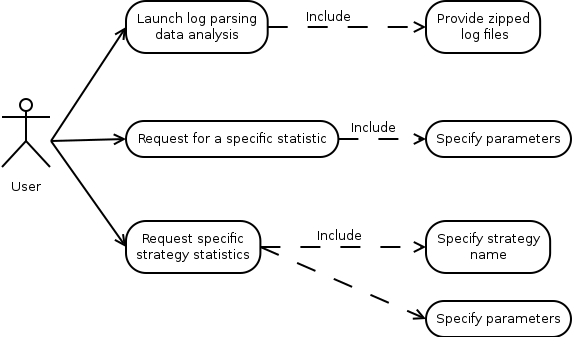
\includegraphics[scale=0.45,keepaspectratio]{diaRessources/UseCaseParsing}\\
Avant l'utilisation de toutes les fonctionnalités du programme, l'utilisateur doit lancer l'analyse.
\subsection{Lancement de l'analyse du log}
\subsubsection{Description et priorité}
\textbf{Niveau de priorité = haute}\\
\begin{itemize}
  \item L'utilisateur devra placer tous les logs compressés (fichiers tar.bz2) destinés à  être analysées dans un dossier spécifique.
  \item si aucune compression n'est donnée la compression par défaut est \textit{snappy}.
    \item Pour des fins de test, afin d'éviter d'avoir un 4 heures étape d'analyse, l'utilisateur peut spécifier un pourcentage des logs pour être analysée. en spécifiant une valeur comprise entre 0 et 100. l'analyseur choisira au hasard les logs de ceux qui sont prévus et les analyser, en créant une base de données utilisable pour des tests supplémentaires.
    \item Une fois que l'analyse est effectuée un message sera affiché sur la console (traitement de fait).

\end{itemize}

\subsection{Statistiques demandées}
\subsubsection{Description et priorité}
\textbf{Niveau de priorité = haute}\\
La demande d'une statistique peut être faite en tapant les états de \textit{dominionmining (paramètres)}.  \\
Les noms de stratégie possibles sont: big money, pen province, beyond silver.\\
Si d'autres stratégies sont reconnues par le programme, ils seront ajoutés à la liste.\\
La liste des paramètres qui seront possible d'utiliser sera déterminée dans le futur.\\

Le retour d'une statistique peut être un graphique affiché dans une fenêtre ou exportés vers un fichier. Si sa une valeur unique, un nom ou une phrase, il sera retourné à l'invite.

\subsection{Mappage des données de jeu}

Afin de permettre à l'utilisateur de demander des statistiques spécifiques concernant un jeu, le programme peut être exécuté afin de générer des logs de jeu simplifiées et un script python sera appliqué à ce log. Cela permettrait une plus grande flexibilité dans le type de statistiques affichables par le programme.
\begin{itemize}
\item Le programme sera lancé en utilisant la commande suivante: \textit{dominionmining data\_to\_query user\_script.py}
 \item Le script python sera appliquée au résultat généré et retourner les statistiques demandées par l'utilisateur.
\item Le fichier généré contenant les résultats de la requête aura le format suivant:
\begin{itemize}
\item Le nom du fichier produit est \textit{game.txt}
\item Le log simplifié contiendra chaque action effectuée par le joueur, une action par ligne. Liste des actions et leur format:
\begin{itemize}
\item Révéler une carte: \textit{joueur\_x révèle carte\_nom}
\item Piocher des cartes: \textit{joueur\_x jete n cartes}
\item Acheter une carte: \textit{joueur\_x buys carte\_name}
\item Jeter des cartes: \textit{joueur\_x trashes n cartes}
\item Mettre une carte \textit{joueur\_x puts carte\_name}
\item Gagner une carte: \textit{joueur\_x gains carte\_name}
\item Jouer une carte: \textit{joueur\_x jouer une carte\_name}

\end{itemize}
\end{itemize}
\end{itemize}
\fi
\subsection{Modélisation des données}
La première démarche consistait à modéliser les données disponibles pour créer une cohérence entre tous les formats existants. Il fallait commencer par décompresser les données, même si, comme on l'a vu, cela ne pouvait être fait que par "tranches" de temps (journées de \textit{Logs}) à cause des ressources mémoire disponibles. 

\subsubsection{Décompression des logs}
\paragraph*{Description et priorité} 



\textbf{Niveau de priorité = haute}



\begin{itemize}
  \item Les fichiers tar.bz2 seront stockés dans un dossier.
  \item Le programme va  décompresser un fichier spécifié à partir de ce dossier dans un dossier temporaire.
  \item Le programme va  supprimer les \textit{Logs} décompressés  à la demande du parser.
\end{itemize}

\subsubsection{Parser}

\paragraph*{Description et priorité} 



\textbf{Niveau de priorité = haute}



Compte tenu des problèmes mis en évidence en analysant un échantillon de \textit{Logs} (comme par exemple des incohérences de syntaxe), l'utilisation d'un parser (comme \textit{YACC} et \textit{LEX}) n'est pas recommandée. C'est pour cette raison que l'on va créer un parser qui utilisera les mots-clés et l'HTML déjà présents dans les \textit{Logs}. Ce parser sera responsable de la lecture et de la collecte des informations importantes sans perdre la structure du \textit{Log}.
Un aperçu des données devant être reconnues par le parser est représenté dans l'illustration suivante :\\


\includegraphics[scale=0.35,keepaspectratio]{diaRessources/UseCaseParser}

\begin{itemize}
\item Winners: liste des gagnants du jeu, il peut y avoir plusieurs gagnants en cas d'égalité.
\item Market: liste des 10 cartes disponibles pour être acheté par les joueurs.
\item Cards Gone: liste des cartes qui ont été entièrement acquises à la fin de la partie.
\item First hand: liste des cartes obtenues au début de partie.%à voir
\item Player Name: Nom du joueur.
\item Victory points: nombre de points à la fin de la partie.
\item Player cards: liste des cartes obtenues à la fin de jeu avec des noms et de quantités differents.
\item Victory cards: liste des cartes de victoire le joueur avec le acheté.
\item Trash: liste des cartes qui sont jetés à la fin de la partie.
\item Game Moves: liste des actions effectuées pendant chaque tour d'un joueur.
\end{itemize}
Le parser doit lire chaque élément montré dans le graphique précédent en tant que partie des données lorsque l'utilisateur exécute le programme de parsing\\

\subsubsection{Créer le game-log}
\paragraph*{Description et priorité}
\textbf{Niveau de priorité = haute}\\
Cette fonctionnalité est la création d'une structure de données où les données du log seront écrites.
Voici une représentation graphique d'une vue d'ensemble de la structure de données:\\
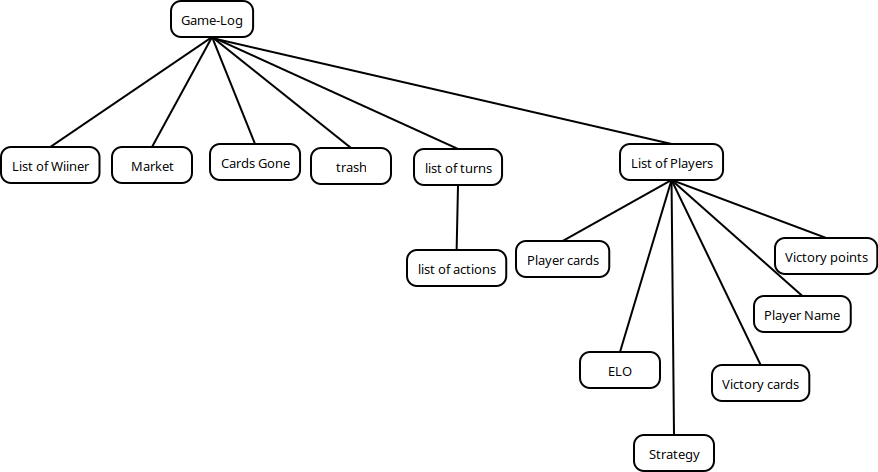
\includegraphics[scale=0.5,keepaspectratio]{diaRessources/game-log}

\subsubsection{Créer une base de données orientée document }

\paragraph*{Description et priorité}
\textbf{Niveau de priorité = haute}\\
Ce module sera responsable de la création de la base de données orientée document, contenant des données au format JSON.
\subsubsection{Se connecter à la base de données orientée document }
\paragraph*{Description et priorité}
\textbf{Niveau de priorité = haute}\\
\begin{itemize}
\item La base de données orientée document sera en charge des échanges à travers un socket spécifique.
\item La base de données orientée document recevra les logs de jeu au format JSON.
\item La base de données orientée document recevra les demandes du programme relatif à chaque élément de données qu'il contient.
\item La base de données orientée document enverra les résultats des demandes effectuées par le programme.
\end{itemize}


\subsubsection{Compression}
\paragraph*{Description et priorité}
\textbf{Niveau de priorité = moyen}\\

La base de données orientée document contiendra la plupart des données et un certain niveau de compression devra être appliquée.
La base de données que nous allons utiliser est focalisée sur mongodb, et elle offre 2 niveaux de compression \textit{Zlib} et \textit{Snappy}.
Au cours du développement \textit{Snappy} est utilisé car il offre une meilleure performance.
Mais le programme final devrait donner à l'utilisateur la possibilité de choisir le niveau de compression lors du démarrage de l'analyse du log.

\subsubsection{Sauvegarder le game-log}

\paragraph*{Description et priorité}
\textbf{Niveau de priorité = haute}\\
\begin{itemize}
\item La base de données orientée document permet de convertir la structure log de jeu dans un document au format JSON.
\item Les données fournies au format JSON seront stockées dans la base de données.
\end{itemize}
%partie de python à discuter
\subsection{Analyse des données}
\subsubsection{Recueillir des données}
\paragraph*{Description et priorité}
\textbf{Niveau de priorité = haute}\\
\begin{itemize}

\item L'analyseur de données va convertir les résultats de la requête dans un format utilisable par le module de plotting.
\item Si les données sont simples à lire (par exemple: un numéro, un nom, une phrase), l'analyseur de données sera tout simplement envoyer le résultat au format texte.
\item La dernière requête sera mémorisée avec son résultat afin de gagner du temps si la prochaine requête faite par l'utilisateur est le même.
\item Si l'utilisateur souhaite appliquer une fonction aux logs de jeu, le programme demandera les logs de jeu et appliquera la fonction a chaque log
\end{itemize}

\subsubsection{restorer le game-log}
\paragraph*{Description et priorité}
\textbf{Niveau de priorité = moyen}\\

Cette fonction est responsable pour restaurer l'information manquante sur les logs analysés, en utilisant la déduction basique sur la base des données obtenues par le log.\\
En cas d'un en-tête du jeu manquant ou partie manquante:
  \begin{itemize}
\item Gagnants / cartes de victoire / points de victoire manquant: le programme peut garder la trace des cartes détenues par les joueurs pendant le jeu afin de savoir combien de cartes victoire qu'ils ont à la fin de la partie.
\item Market manquant: Le programme peut garder la trace des cartes achetées au cours du jeu afin de reconstituer partiellement ou totalement les cartes disponibles sur Market.
\item Cartes Gone: Comme avec les données manquantes de Market, le programme permet de garder une trace de cartes achetées et compter la quantité achetée pour chaque carte, si le montant maximum de cartes est acheté, la carte a disparu à la fin de la partie.
\item Nom du joueur manquant: le jeu se déplace partie d'un log assure également le suivi des noms des joueurs, le programme sera tout simplement de les restaurer dans l'en-tête.
\item Cartes de joueur: le programme permet de garder une trace des actions effectuées au cours du jeu par rapport aux cartes de joueurs et les ajouter dans cette liste.
  \end{itemize}

\iffalse
\subsubsection{Plotting}
\paragraph*{Description et priorité}
\textbf{Niveau de priorité = haute}\\

Le module de plotting va obtenir les données converties obtenues après le processus de recueillir des données et de les tracer dans une interface graphique. Ce module va fonctionner d'une manière similaire de \textit{GnuPlot}.
\fi

\subsubsection{Calculer l'\textit{\textbf{ELO}}}
%TODO
\paragraph*{Description et priorité}
\textbf{Niveau de priorité = haute}\\

L'analyseur devra calculer l'ELO final de chaque joueur ainsi que son ELO temporaire à l'issue d'une partie.\newline
pour chaque partie dans l'ordre chronologique, l'analyseur demandera l'ELO initial de ce joueur grace aux données générales du joueur. L'analyseur va ensuite calculer l'ELO de chaque joueur à l'issue de cette partie et les ajouter aux données relatives au log en question et va également mettre à jour l'ELO général des joueurs concernés dans leurs données générales afin de pouvoir continuer à calculer leur évolution.

Plus d'informations sur ELO peuvent être consultés sur \url{https://en.wikipedia.org/wiki/Elo_rating_system}\\
\iffalse
%TODO: refaire le diagramme du calcul de l'elo
Le schéma suivant illustre le processus du calcul de elo:\\
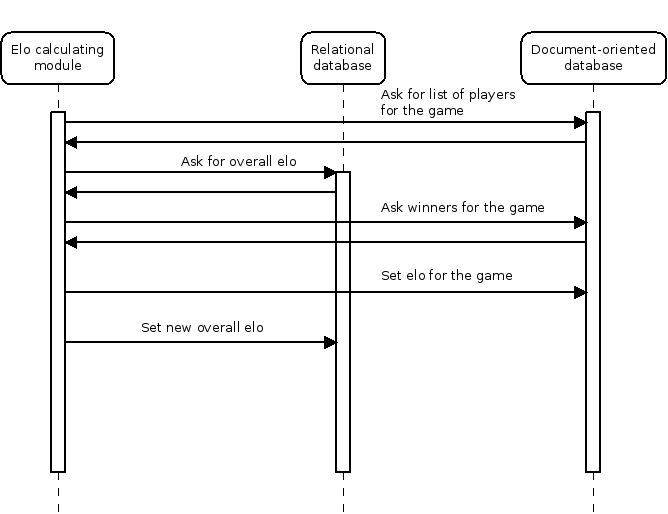
\includegraphics[width=\textwidth,height=\textheight,keepaspectratio]{diaRessources/elocalc}\\
\fi
\subsubsection{Reconnaître les stratégies}
\paragraph*{Description et priorité}
\textbf{Niveau de priorité = moyen}\\

Le wiki de dominion décrit quelques stratégies qui peuvent être utilisés dans le jeu.\\Par exemple :\\
Big Money\\
Beyond Silver\\
Penultimate Province Rule\\
Pour plus de détails sur \url{http://wiki.dominionstrategy.com/index.php/Strategy}\\



\textbf{Cette image décrit le processus de décision associé à la stratégie Big Money}\\
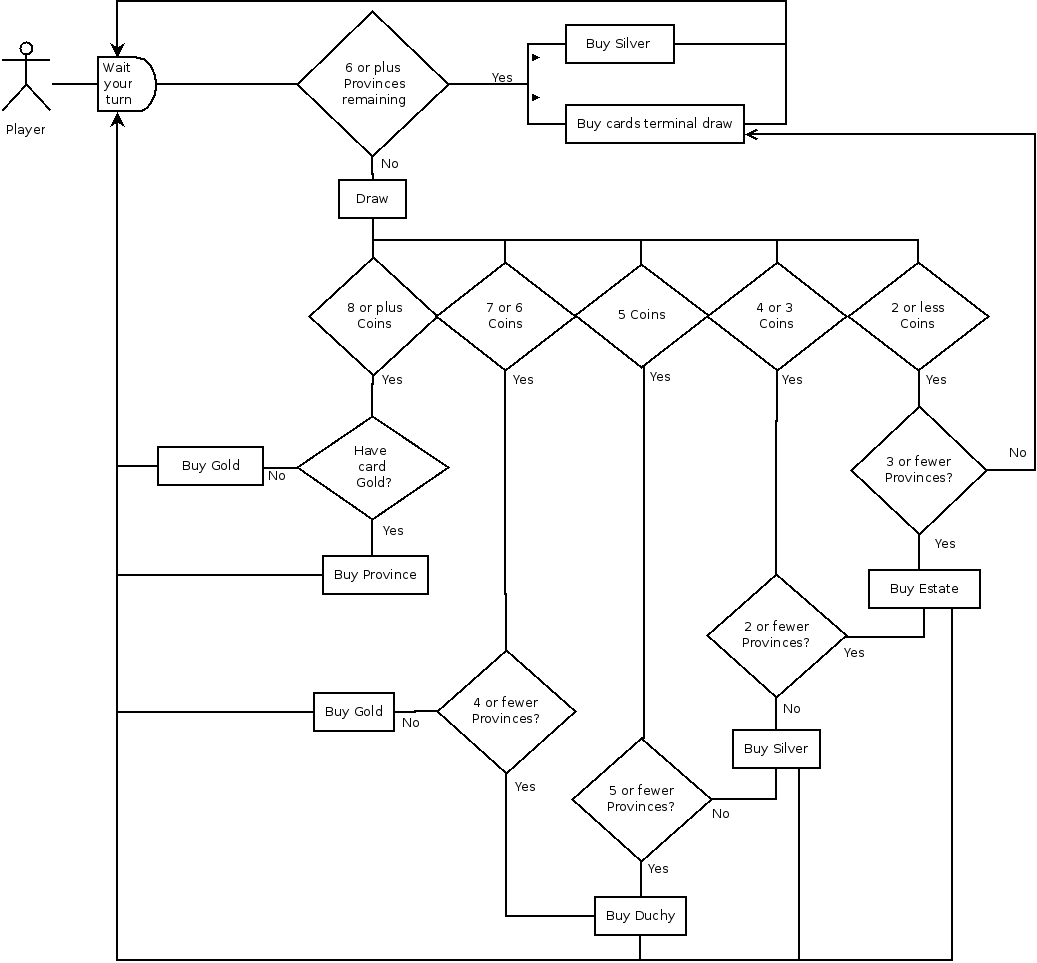
\includegraphics[width=\textwidth,height=\textheight,keepaspectratio]{diaRessources/big-money}\\
%The analyzer has to recognize when a player buys only money cards and specific cards related to the big money strategy. It also has to keep track of the remaining provinces to be bought.\\
L'analyseur devra être en mesure de reconnaître quelle stratégie a été utilisée sur un match donné (si une  stratégie a été utilisée) et générer des statistiques.\\
Plus de détails \url{http://wiki.dominionstrategy.com/index.php/Big_Money}\\

Afin de reconnaître la stratégie Beyond Silver ou Big Money, l'analyseur doit reconnaître lorsque certains types de cartes sont achetées, la liste de ces cartes peuvent être trouvée sur : \url{http://wiki.dominionstrategy.com/index.php/Silver#Beyond_Silver} et \url{http://wiki.dominionstrategy.com/index.php/Big_Money}\\

Afin de reconnaître que Penultimate Province Rule est respecté (comme expliqué à \url{http://dominionstrategy.com/2011/03/28/the-penultimate-province-rule/}), l’analyseur doit garder une trace de la quantité de Points de Victoire de chaque joueur à chaque tour.

\subsubsection{Reconnaître le Greening}
\paragraph*{Description et priorité}
\textbf{Niveau de priorité = haute}\\

L'analyseur doit être capable de reconnaître le moment de \textit{\textbf{greening}} sur chaque match.
En savoir plus à propos de \textit{\textbf{greening}} sur \url{http://wiki.dominionstrategy.com/index.php/Greening}.\\
Le programme va reconnaître quand le greening commence en détectant lorsque les cartes de victoire commencent à être achetées.

\newpage

\section{Besoins non-fonctionnels}

\subsection{Besoins de performance}

Aucun besoin de performance spécifique n’a été fait par le client. Mais pour l'analyseur le temps d’exécution  doit être inférieur à une heure.\\
L'utilisateur doit être capable de parcourir le processus d'analyse sur un ensemble de données précis sans devoir attendre que la même requête soir refaite.

\subsection{Fiabilité}
Le client demande qu'un maximum de logs soient récupérés, la totalité des logs ne pourra pas être parsé mais une marge de 5 à 10\% de logs peut être ignorée.\newline
En revanche lorsque un log est parsé, le programme devra récuperer 100\% des données présentes de celui-ci et si possible restaurer les informations non présentes dans le log de départ.
\subsection{Attributs de qualité de logiciels}

Le programme devra pouvoir lancer la phase initiale de parsing en une seule ligne de commande.\\
Les fonctions présentes dans la librairie à l'attention de l'utilisateur devront avoir un nom clair et facile à comprendre.\\
Les données générées par l'analyseur n’ont pas besoin à être lisibles par l'homme.\\
Les game log générés devront pouvoir être analysés par l'utilisateur afin de permettre la plus grande souplesse possible dans le traitement des logs.

\section{Besoins organisationnels}

La répartition des tâches du projet et l'estimation de la durée de chacune d'elle sont présentées sur le planning suivant:\\

\subsection{Planning prévisionnel}

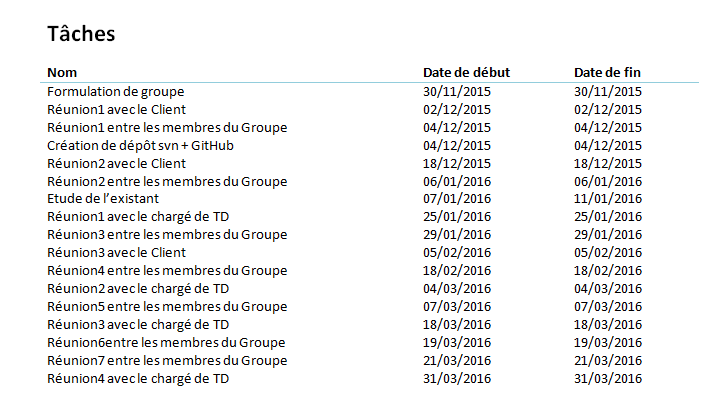
\includegraphics[scale=0.45,keepaspectratio]{planning}\\

\subsection{Diagramme de Gantt}

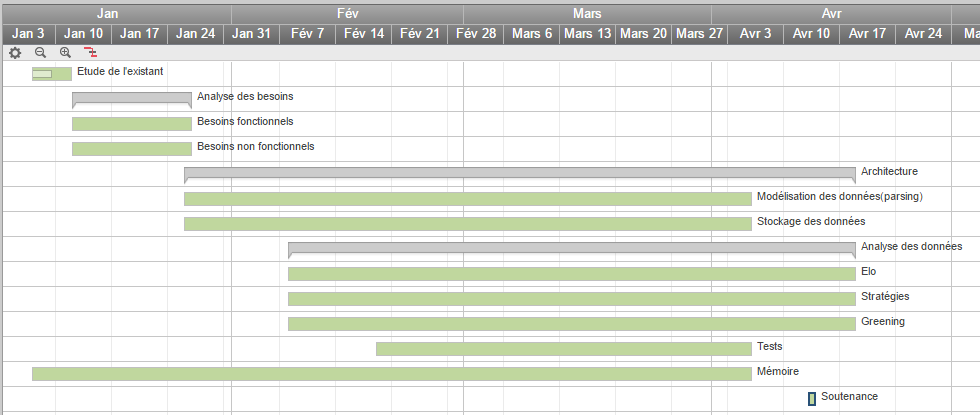
\includegraphics[scale=0.45,keepaspectratio]{gantt}\\

\newpage
\iffalse
\section{Développement}

Intro

\subsection{Tâches}

Bla\\


%tableau à taille fixée sur certaines colonnes (param sur la ligne \begin{tabularx}, voir wiki pour plus d'info sur la syntaxe
\begin{figure}[!h]
\begin{center}
\begin{tabularx}{17cm}{|c|p{6cm}|X|}
  \hline
  Priorité & Nom & Raison\\
  \hline
  1 & Tache 1 & Doit être vérifié en premier car sinon [...] \tabularnewline
  2 & Tache 2 & On doit pouvoir [...] \tabularnewline
  3 & Tache 3 & Comme les principales fonctionnalités permettant de tester sont opérationnelles, nous pouvons passer à cette tâche. \tabularnewline
  4 & Tache 4 & Parce que [...] \tabularnewline
  5 & Tache 5 & La tache 5 fait partie des principales [...]. \tabularnewline
  6 & Tache 6 & Dernière fonctionnalité essentielle à mettre en place. \tabularnewline
  7 & Tache 7 & Non-essentiel, mais apporterait un plus au projet. \tabularnewline
  8 & Tache 8 & Non-essentiel, mais apporterait un plus au projet. \tabularnewline
  \hline
\end{tabularx}
\end{center}
\caption{Tableau récapitulatif des tâches}
\end{figure}

\subsection{Tests}

Bla\\

\begin{figure}[!h]
\begin{center}
\begin{tabularx}{17cm}{|p{6cm}|X|}
  \hline
  Fonctionnalité & Test\\
  \hline
  Fonction 1 & Quand [...], vérifier [...]. \tabularnewline
  & Et quand [...], vérifier [...]. \tabularnewline
  Fonction 2 & Vérifier [...]. \tabularnewline
  Fonction 3 & Vérifier [...]. \tabularnewline
  Fonction 4 & Avoir [...]. \tabularnewline
  Fonction 5 & Accéder à [...]. \tabularnewline
   & Vérifier que [...]. \tabularnewline
  Fonction 6 & Accéder à [...]. \tabularnewline
   & Et vérifier [...]. \tabularnewline
  Fonction 7 & Installer [...]. \tabularnewline
   & Vérifier [...]. \tabularnewline
  Fonction 8 & Compter [...]. \tabularnewline
  \hline
\end{tabularx}
\end{center}
\caption{Tableau récapitulatif des tests}
\end{figure}
\fi


\chapter{Architecture et description du logiciel}
Dans cette partie, nous allons d'abord vous parler de la partie concernant le parsing puis passer à la partie d'analyse des données et de rendu graphique.

\section{Partie parser}
Cette partie est écrite en java, l'autre possibilité que nous avions était de coder le parser en python mais après quelques petits tests nous nous sommes rendus compte que le parser en python serait beaucoup trop lent. Voici l'architecture de la partie Java de notre projet:
%TODO: ajouter une image de l'architecture java
%\includegraphics{}

En raison de logs au format variable, il est nécessaire de produire plusieurs versions de parser afin de garder une robustesse au niveau du parsing et d'éviter une classe trop grosse. Pour cela, à l'ouverture d'un log, le LogHandler demande la création d'un parser à une classe utilisant le design pattern factory. Cette classe va examiner le log en question et choisir la bonne version du parser a utiliser puis renvoyer ce parser au log handler. Afin d'éviter des duplications de code inutiles, le parser en lui même est implémenté à l'aide d'une classe abstraite regroupant toutes les similitudes entre les parsers puis les différences sont implémentées dans la classe du parser en question à proprement parler. Le LogHandler va ensuite envoyer sur une base de données les données obtenues à l'aide du parser.

\section{Partie Analyse}
Cette partie est écrite en python à la demande du client. Nous avons choisi de proposer plusieurs librairies contenant des outils besiques permettant de travailler sur les données acquises lors du parsing. Voici un schéma regroupant les différentes librairies et leurs liens:
%TODO: ajouter une image de l'architecture python
%\includegraphics{}
Tout d'abord, le module MongoInterface permet de communiquer avec la base de données.\newline
Les objets Matchs et Player sont utilisés lors de la récupération de données afin de le mettre en forme pour une utilisation plus aisée par le client. Ce sont des structures de données regroupant toutes les information relatives au match ou joueur en question.\newline
La bilbiothèque Tools regroupe les fonctions d'analyse basique pouvant être utilisées sur les logs, pour appliquer ces fonctions, il faut utiliser la fonction \textit{apply\_function\_to\_query}. Si dans le futur, le client ou bien des personnes souhaitant travailler sur ce projet veulent étoffer les fonctions proposées, il suffira de les ajouter dans cette libraire.\newline
La solution proposée pour afficher les resultats consiste en un module Plotter et un module DataSet. Le module DataSet permet de mettre en forme les données à représenter de manière simple pour l'utilisateur, et le module Plotter propose une solution simple pour afficher des résultats de base (lignes cassées, nuage de points ou barres).

\section{Extensions possibles}
Sur la partie parser, il est très facile d'ajouter une nouvelle version de parser permettant de lire par exemple des logs d'un nouvelle version du serveur de jeu, cela permettrait de regouper des données sur une plus grande période et donc d'obtenir des statistiques plus intéressantes.\newline
Sur la partie Python, il est possible d'ajouter de nouvelles fonctions d'analyse des données, des données peuvent également être rajoutées pour les logs mais il faudra faire attention à la lecture de ces données car les objets ne permettrons pas un accès facile à celles-ci (sauf si l'utilisateur modifie également les structures de données).


Dans cette partie nous cherchons à décrire dans un premier temps [...], puis, c[...].

\section{Partie 1}

Intro

\subsection{Sous-partie 1}

\begin{figure}[!ht]
\begin{center}

\includegraphics[height=12cm]{autre_partie/image1}
\end{center}
\caption[autre partie générale]{autre partie image 1\protect\footnotemark}
%\floatfoot{Source: (Citation command)}
% avec le package "floatrow"
\end{figure}

%footnote protected pour apparaitre dans la légende d'une image
\footnotetext{Schéma d'après : \textit{Auteur 1 \& Propriétaire image}, LICENCE (cf. ref. \cite{cite4})}

\newpage{}

\subsection{Sous-partie 2}

\begin{figure}[!ht]
\begin{center}

\includegraphics[height=12cm]{autre_partie/image2}
\end{center}
\caption[autre partie]{autre partie globale de notre quelque chose}
\end{figure}

Nous retrouvons ici, blabla\footnote{Application bla - Interface blabla} [...].

\subsubsection{Sous-sous-partie 1}

Le bla (cf. ref. \cite{cite6}) est [...]:

\begin{itemize}
\item item1;
\item item2;
\item item3;
\item item4;
\item item5.
\end{itemize}

\newpage

\subsubsection{Sous-sous-partie 2}

%Les lignes :
% \setcounter{secnumdepth}{4}
% \setcounter{tocdepth}{4}
%dans le fichier "main.tex" permettent de faire en sorte que les paragraphes soient interprété comme des titres de niveau 5
\paragraph{Paragraphe 1 (agissant comme titre niveau 5)}
%forcer un saut de ligne
~\\
\hskip7mm

\begin{figure}[!ht]
\begin{center}

\includegraphics[height=6cm]{autre_partie/image3}
\end{center}
\caption[Structure d'unz autre chose]{Structure d'une autre chose\protect\footnotemark}
\end{figure}

Ce schéma représente bla.

\footnotetext{Schéma et explication d'après le wiki bla (cf. ref. \cite{cite0})}

\paragraph{Paragraphe 2}
~\\
\hskip7mm

%fixer les floats précédemment définis
%\FloatBarrier

Bla

\subparagraph{Sous-paragraphe 1}
~\\
\hskip7mm

Bla

\begin{figure}[H]
\begin{center}

\includegraphics[height=10cm]{autre_partie/image4}
\end{center}
\caption{Diagramme de truc}
\end{figure}

\subparagraph{Sous-paragraphe 2}
~\\
\hskip7mm

Bla\\

Bla

\subparagraph{Sous-paragraphe 3}
~\\
\hskip7mm

Bla

\subsubsection{Sous-sous-partie 3}

Bla

\section{Partie 2}

Bla

\footnotetext{D'après le schéma disponible sur la documentfation officielle disponible sur le site blalbla}

Bla

\subsection{Sous-partie 1}

Bla

\subsection{Sous-partie 2}

Bla

\paragraph*{Paragraphe 1 (n'apparaitra pas dans l'index)}
Bla

\paragraph*{Paragraphe 2}
Bla

\paragraph*{Paragraphe 3}
Bla

\subsection{Sous-partie 3}

Bla




\chapter{Fonctionnement et Tests}

Dans cette partie nous allons tout d'abord nous pencher sur le fonctionnement et les tests concernant la partie parser du projet, puis nous allons aborder les mêmes points pour la partie analyse des données.

\section{Parser}

Cette partie du projet est écrite en java, nous avons utilisé JUnit afin de mener à bien ces tests unitaires. De plus le dépôt git est muni d'un outil d'intégration continue (Travis) qui est assoscié à nos tests afin de garantir que le développement ne produit pas d'erreurs sur le fonctionnement du programme. \\

De plus nous avons effectué des tests de couverture en utilisant le plugin Cobertura Maven qui nous a aidé à détecter les points plus faibles au niveau des tests et ainsi proposer d'autres tests unitaires pour avoir une meilleur couverture.


\subsection{Politique de tests}

Du fait de l'utilisation de java, pour chaque classe non-utilitaire un premier test vérifie systématiquement que la création des objets fonctionne correctement, une fois ce critère validé, des tests spécifiques à chaque classe sont effectués en fonction des fonctionnalités qu'elles remplissent.\\

Le but de nos test est de verifier l'extraction des donnéees des logs, pour cela, nous avons choisi deux logs réels représentatifs de chaque version et avons appliqué la stratégie suivante:  \\
En premier lieu nous avons réalisé des test pour verifier la bonne detection de la version pour les différents types de version. \\
Ensuite nous avons pris chaque donnée de la structure et avons validé qu'elle ne soit pas vide, dans le cas où l'élément est une liste, nous vérifions que le nombre d'éléments correspond, et finalement pour les éléments carte/quantité, comme par exemple \textit{victory cards} ou \textit{market} nous vérifions que le couple nom, valeur corresponde.

\subsection{Tests unitaires}



\subsection{Tests de couverture}
%TODO: ajouter les images pour les tests de couverture
Nous n'avons pas pu effectuer de tests pour la classe LogHandler par manque de temps.\\ Le test de conversion du document dans le serveur MongoDb vers l'objet n'est pas nécesssaire car le parser se contente d'ajouter des éléments vers la base de données sans jamais récupérer des données déja écrite. Dans le cas ou l'évolution du projet amènerait à des lectures de données depuis la partie Java, il faudra créer ce test.

\section{Bugs rencontrés}

\paragraph*{Dictionnaire de Cartes} 

Il existe une classe qui sert à verifier l'existence d'une carte et returne en même temps le nom générique de la carte donnée.\\
Il y a des problèmes avec les cartes dont le pluriel change radicalement du singulier. par exemple les cartes Colonies (Colony) et Duchies (Duchy). \\

Pour resoudre le bug il faut changer le dictionaire actuelmement implementé, pour ajouter la convertion de cartes en pluriel qui sont des cas atypiques.

Pour la classe logReaderAbs, il y a des actions qui ne sont pas testées car, dans les logs selectionnés pour les tests il n'existe pas toutes les actions possibles pour les Joueurs, une solution serait de modifier le .

\paragraph*{Nom de Joueurs} 

Dans les logs nous avons trouvé des noms de joueurs très dificiles à traiter car ils ont beaucoup de caractères spéciaux ainsi que des noms explicitement ecrits pour casser des programmes,
par exemple System.out.println("hola"), ou ;) ou même , des noms avec des mots reservés pour les langages de programmation.


\section{Module d'analyse des donnée}
Cette partie du projet écrite en Python est cruciale car c'est ce qui sera utilisé par l'utilisateur. Nous avons utilisé le module unittest pour effectuer nos tests unitaires ainsi que mongomock pour simuler l'utilisation d'un serveur MongoDB. Les tests de couverture ont été effectués à l'aide de pytest

\subsection{Politique de tests}
Nous avons testé le module Match et Tools afin de vérifier leur bon fonctionnement, les tests effectués sont des tests unitaires. Pour effectuer nos tests, nous avons produit un log prédéfini a comparer au résultat des tests effectués.

\subsection{Tests unitaires}
\paragraph{module Match}
Trois tests unitaires ont été effectués:
\begin{itemize}
\item un test de comparaison du nom des joueurs.
\item un test de comparaison du log a proprement parler, c'est à dire les actions des joueurs au cours de la partie
\item un test de comparaison des informations du header.
\end{itemize}

Ces trois tests passent sans poser de problèmes.

\paragraph{Module Tools}
Trois tests unitaires ont été effectués:
\begin{itemize}
\item un premier test permet de vérifier la bonne crétation de la pseudo base de données (utilisation de mongomock).
\item un second test vérifie la bonne création des informations gloabales pour chaque joueur présent dans le log test (2 joueurs).
\item le troisième test vérifie que la fonction de calcul d'elo s'applique correctement ainsi que la détection du \textit{greening}.
\end{itemize}

\subsection{Tests de couverture}
Le résultat des tests de couverture est le suivant:\\
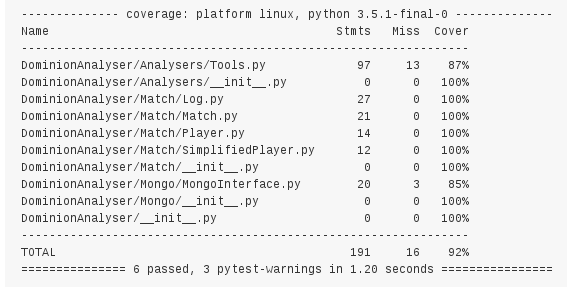
\includegraphics[scale=0.35,keepaspectratio]{./coverage_python_code}
Nous ne couvrons pas totalement le module Tools, cela s'explique par le fait que nous n'avons pas fait de tests sur la reconaissance des stratégies.\\
Le module MongoInterface n'est pas entièrement couvert non plus, car nous ne testons pas la création d'index et de collections.


\paragraph{conclusions}
Par manque de temps, nous n'avons pas pu effectuer plus de tests mais une suite logique à ces quelques tests unitaires serait de produire des logs pouvant poser problème, par exemple avec des caractères spéciaux ou bien des mots clefs relatifs au langage python. Concernant les test unitaires des outils, d'autres tests pourraient être effectués pour la detection des stratégies ou bien pour des valeurs d'ELO ambigües.



\subsection{Bugs rencontrés}
Du fait du peu de tests, nous n'avons pas rencontré de bugs sur ces tests mais les pistes évoquées dans la partie tests de couverture ne manqueront pas de révéler des faiblesses potentielles dans le code produit.

\iffalse
\subsection*{Sous-partie 1 ('apparaitra pas dans l'index)} Bla



\paragraph*{Paragraphe 3} Bla

\newpage

\subsection*{Sous-partie 2}

Bla

%galerie d'image
\begin{figure}[htp]
  \centering
  \subfloat[Première image]{\label{fig:première}
\includegraphics[scale=0.8]{resultats/gallerie}}
  ~ %espace entre deux images sur une même ligne
  \subfloat[Deuxième image]{\label{fig:deuxième}
\includegraphics[scale=0.8]{resultats/gallerie}}
  ~
  \subfloat[Troisième image]{\label{fig:troisième}
\includegraphics[scale=0.8]{resultats/gallerie}}
  ~\\ %saute une ligne dans la galerie d'image
  \subfloat[Quatrième image]{\label{fig:quatrième}
\includegraphics[scale=0.8]{resultats/gallerie}}
  ~
  \subfloat[Cinquième image]{\label{fig:cinquième}
\includegraphics[scale=0.8]{resultats/gallerie}}
  \caption{Différents screenshots quelque chose, en gallerie}
  \label{fig:gallerie1}
\end{figure}
\fi


\chapter{Autre partie}

Dans cette partie nous cherchons à décrire dans un premier temps [...], puis, c[...].

\section{Partie 1}

Intro

\subsection{Sous-partie 1}

\begin{figure}[!ht]
\begin{center}

\includegraphics[height=12cm]{autre_partie/image1}
\end{center}
\caption[autre partie générale]{autre partie image 1\protect\footnotemark}
%\floatfoot{Source: (Citation command)}
% avec le package "floatrow"
\end{figure}

%footnote protected pour apparaitre dans la légende d'une image
\footnotetext{Schéma d'après : \textit{Auteur 1 \& Propriétaire image}, LICENCE (cf. ref. \cite{cite4})}

\newpage{}

\subsection{Sous-partie 2}

\begin{figure}[!ht]
\begin{center}

\includegraphics[height=12cm]{autre_partie/image2}
\end{center}
\caption[autre partie]{autre partie globale de notre quelque chose}
\end{figure}

Nous retrouvons ici, blabla\footnote{Application bla - Interface blabla} [...].

\subsubsection{Sous-sous-partie 1}

Le bla (cf. ref. \cite{cite6}) est [...]:

\begin{itemize}
\item item1;
\item item2;
\item item3;
\item item4;
\item item5.
\end{itemize}

\newpage

\subsubsection{Sous-sous-partie 2}

%Les lignes :
% \setcounter{secnumdepth}{4}
% \setcounter{tocdepth}{4}
%dans le fichier "main.tex" permettent de faire en sorte que les paragraphes soient interprété comme des titres de niveau 5
\paragraph{Paragraphe 1 (agissant comme titre niveau 5)}
%forcer un saut de ligne
~\\
\hskip7mm

\begin{figure}[!ht]
\begin{center}

\includegraphics[height=6cm]{autre_partie/image3}
\end{center}
\caption[Structure d'unz autre chose]{Structure d'une autre chose\protect\footnotemark}
\end{figure}

Ce schéma représente bla.

\footnotetext{Schéma et explication d'après le wiki bla (cf. ref. \cite{cite0})}

\paragraph{Paragraphe 2}
~\\
\hskip7mm

%fixer les floats précédemment définis
%\FloatBarrier

Bla

\subparagraph{Sous-paragraphe 1}
~\\
\hskip7mm

Bla

\begin{figure}[H]
\begin{center}

\includegraphics[height=10cm]{autre_partie/image4}
\end{center}
\caption{Diagramme de truc}
\end{figure}

\subparagraph{Sous-paragraphe 2}
~\\
\hskip7mm

Bla\\

Bla

\subparagraph{Sous-paragraphe 3}
~\\
\hskip7mm

Bla

\subsubsection{Sous-sous-partie 3}

Bla

\section{Partie 2}

Bla

\footnotetext{D'après le schéma disponible sur la documentfation officielle disponible sur le site blalbla}

Bla

\subsection{Sous-partie 1}

Bla

\subsection{Sous-partie 2}

Bla

\paragraph*{Paragraphe 1 (n'apparaitra pas dans l'index)}
Bla

\paragraph*{Paragraphe 2}
Bla

\paragraph*{Paragraphe 3}
Bla

\subsection{Sous-partie 3}

Bla

\chapter{Résultats}

\section{Partie 1}

Intro

\subsection{Sous-partie 1}

\paragraph*{Paragraphe 1 (n'apparaitra pas dans l'index)} Bla

\paragraph*{Paragraphe 2} Bla

\paragraph*{Paragraphe 3} Bla

\subsection{Sous-partie 2}

Bla

\subsection{Sous-partie 3}

Bla

\section{Partie 2}

Intro

\subsection*{Sous-partie 1 ('apparaitra pas dans l'index)} Bla

\paragraph*{Paragraphe 1 ('apparaitra pas dans l'index)} Bla

\paragraph*{Paragraphe 2} Bla

\paragraph*{Paragraphe 3} Bla

\newpage

\subsection*{Sous-partie 2}

Bla

%galerie d'image
\begin{figure}[htp]
  \centering
  \subfloat[Première image]{\label{fig:première}
\includegraphics[scale=0.8]{resultats/gallerie}}
  ~ %espace entre deux images sur une même ligne
  \subfloat[Deuxième image]{\label{fig:deuxième}
\includegraphics[scale=0.8]{resultats/gallerie}}
  ~
  \subfloat[Troisième image]{\label{fig:troisième}
\includegraphics[scale=0.8]{resultats/gallerie}}
  ~\\ %saute une ligne dans la galerie d'image
  \subfloat[Quatrième image]{\label{fig:quatrième}
\includegraphics[scale=0.8]{resultats/gallerie}}
  ~
  \subfloat[Cinquième image]{\label{fig:cinquième}
\includegraphics[scale=0.8]{resultats/gallerie}}
  \caption{Différents screenshots quelque chose, en gallerie}
  \label{fig:gallerie1}
\end{figure}



\newpage

%récupérer les citation avec "/footnotemark"
\nocite{*}

%choix du style de la biblio
\bibliographystyle{plain}
%inclusion de la biblio
\bibliography{bibliographie}
%voir wiki pour plus d'information sur la syntaxe des entrées d'une bibliographie

\end{document}
